%!TEX root = ../main.tex

%%%%%%%%%%%%%%%%%%%%%%%%%%%%%%%
%%%%%%%%%%%%%%%%%%%%%%%%%%%%%%%
\chapter{Fundamentals}
% Evtl. lieber Basics nennen; Stand der Technik ist es ja nicht wirklich
\label{chap:fundamentals}

\commenting{Input of basic knowledge for system modelling; Maybe supplementary knowledge} % \mycomment[MK]{Write Chap Fundamentals}

General sources in terms of standard literature: \autocite{oedingElektrischeKraftwerkeUnd2016,gloverPowerSystemAnalysis2017,kundurPowerSystemStability2022,machowskiPowerSystemDynamics2020}

%%%%%%%%%%%%%%%%%%%%%%%%%%%%%%%
\section{Basics synchronous generators}
\label{sec:basics-sg}
\commenting{
        \begin{itemize}
                \item characteristics of a synchronous generator; structure and types of SG's
                \item mathematical background and description of the behavior -> dynamic modelling
                \item \textbf{Swing equations}
        \end{itemize}
}

The final swing equation system can be derived to following two equations, which have to be solved in every time step to determine the pole angle $\delta$ and the rotor speed $\omega$, respectively the rotor speed change from its base value $\Delta\omega$:
\begin{align}
        \frac{d\delta}{dt}&=\Delta\omega \label{eq:swing1} \\[12pt]
        \frac{d\Delta\omega}{dt}&=\frac{1}{2 \cdot H_\mathrm{gen}} \cdot (P_\mathrm{m} - P_\mathrm{e}) \label{eq:swing2}
\end{align}
% where

% \begin{tabularx}{\textwidth}[H]{ll}
%         $\delta$                & power angle \\
%         $\Delta\omega$          & change of rotor angular speed \\
%         $H_\mathrm{gen}$        & inertia constant of the \acs{SG} \\
%         $P_\mathrm{m}$          & mechanical power of the turbine \\
%         $P_\mathrm{e}$          & electrical power demanded transferred out of the \acs{SG}
% \end{tabularx}
% \vspace{12pt}

The generation of a \ac{TDS} for this equation system takes place in \autoref{sec:tds}.

%%%%%%%%%%%%%%%%%%%%%%%%%%%%%%%
\section{System stability esp. transient context}
\commenting{
        \begin{itemize}
                \item What is to be analyzed? And why? -> different stability analysis
                \item rotor angle stability,
                \item \textbf{derivation of EAC,}
                \item basic assessment models (single machine infinite bus, see \autocite{kundurPowerSystemStability2022})
        \end{itemize}
}

With respect to the limitations, that
\begin{enumerate}
        \item the machine is operating under balanced three-phase positive-sequence conditions,
        \item the machine excitation is constant, 
        \item the machine losses, saturation, and saliency are neglected,
\end{enumerate}
a simplified \acf{SMIB} model can be considered for transient stability assessment (see \autoref{fig:smib-model}).  The \ac{IBB} is working with a constant voltage $E_\mathrm{ibb}$ and angle $\delta_\mathrm{ibb}$, typically set to $0^\circ$. The real power flowing from the \ac{SG} to the \ac{IBB} is then expressed within the \autoref{eq:p_e} and only dependent on the power angle $\delta$. The reactance $X_\mathrm{res}$ is expressing the simplified reactance from the respective circuit.
\begin{align}
        P_\mathrm{e}=\frac{E_\mathrm{p} \cdot E_\mathrm{ibb}}{X_\mathrm{res}} \cdot sin(\delta) \label{eq:p_e}
\end{align}
The mechanical power of the turbine is assumed constant, due to the short occurance of transient stability problems.

\begin{figure}[h]
        \centering
        \vspace{1cm}
        \begin{circuitikz}[european, scale=.9, smallR/.style={resistor,resistors/scale=.7}]
            \draw (0,0) node[oscillator, anchor=east, name=gen]{} --(.5,0)
                to[L, name=X_g] ++(2,0) coordinate(f1)
                \bushere{1}{$\underline{E}_\mathrm{T}'$}{}
                to[oosourcetrans,prim=delta,sec=wye] ++(2,0)
                \bushere{1.25}{$\underline{E}_\mathrm{T}''$}{} coordinate(b1) ++(0,-.5) -- coordinate(f2) ++(1.5,0)
                to[L, name=X_l2] ++(1,0) -- ++(1.5,0) ++(0,.5)
                \bushere{1.25}{$\underline{E}_\mathrm{ibb}$}{} ++(0,.5) coordinate(b2) ++(0,-.5) -- coordinate(f3) ++(1,0)
                node[gridnode, anchor=left, name=ib]{};
            \draw (b1) ++(0,.5) to[L, name=X_l1] (b2);
            % \draw[line width=2pt] (2.25,1) -- (2.25,-1);
            % \draw[line width=2pt] (4.75,1) -- (4.75,-1);
            % \draw[line width=2pt] (8.25,1) -- (8.25,-1);
            \node[above=6pt] at (X_g) {$X_\mathrm{g}'$};
            \node[above=6pt] at (X_l1) {$X_\mathrm{l}$};
            \node[below=6pt] at (X_l2) {$X_\mathrm{l}$};
            \path[->] (-1.2,.5) edge [bend right] node[left=6pt]{$E_\mathrm{p}~\angle~\delta$} (-1.2,-.5);
            \path[->] (ib) ++(.8,.5) edge [bend left] node[right=6pt]{$E_\mathrm{ibb}~\angle~0^{\circ}$} ++(0,-1);
            \draw[-Stealth, very thick, red] (f1) ++(0,-.5) -- ++(-.15,-.45) -- ++(.3,.2) -- ++(-.2,-.6) coordinate(f1_text);
            \node[below, red] at (f1_text) {\scriptsize fault 1};
            \draw[-Stealth, very thick, red] (f2) ++(0,.3) -- ++(-.15,-.45) -- ++(.3,.2) -- ++(-.2,-.6) coordinate(f2_text);
            \node[below, red] at (f2_text) {\scriptsize fault 2};
            \draw[-Stealth, very thick, red] (f3) ++(0,.3) -- ++(-.15,-.45) -- ++(.3,.2) -- ++(-.2,-.6) coordinate(f3_text);
            \node[below, red] at (f3_text) {\scriptsize fault 3};
        \end{circuitikz}
        \vspace{.5cm}
        \caption[Representative circuit of a \acf{SMIB} model]{Representative circuit of a \acf{SMIB} model with pole wheel voltage $E_\mathrm{p}~\angle~\delta$ and \acf{IBB} voltage $E_\mathrm{ibb}~\angle~0^{\circ}$; positions of considered faults 1 to 3 are marked with red lightning arrows}
        \label{fig:smib-model}        
\end{figure}
% where

% \begin{tabularx}{\textwidth}[H]{lX}
%         $\delta$                        & power angle \\
%         $E_\mathrm{p}$                  & pole potential of the \acf{SG} \\
%         $\underline{E}_\mathrm{T}'$     & complex potential on the primary side of the transformer \\
%         $\underline{E}_\mathrm{T}''$    & complex potential on the secondary side of the transformer \\
%         $\underline{E}_\mathrm{ibb}$    & complex pole potential of the \acf{IBB} \\
%         $X_\mathrm{g}'$                 & reactance of the \acf{SG} \\
%         $X_\mathrm{l}$                  & reactance of a single line \\
% \end{tabularx}

%%%%%%%%%%%%%%%%%%%%%%%%%%%%%%%
\section{Events harming the system stability}
\commenting{
        \begin{itemize}
                \item \textbf{fault types,}
                \item load-changes
                \item effects of electrical networks (esp. generator networks) vs. single machine systems -> paper \autocite{batchuComparativeStudyEqual2022}: IBB not that extremely fixed, group of critical and non-critical machines; but more of an outlook and targeting real-time calculation (for system operation)
        \end{itemize}
}

The electrical energy system or network is a balance of power input (generation) and output (use). Changes and dynamics of this balance lead to system answers, which can result in a remaining stable system, or unlikely an unstable system. When specifically the generator is moving into an unstable operation, and can not stay in synchronous and stable speed with the rest of the system, it has to be disconnected from the power grid.

\begin{figure}[h]
        \centering
        \vspace{12pt}
        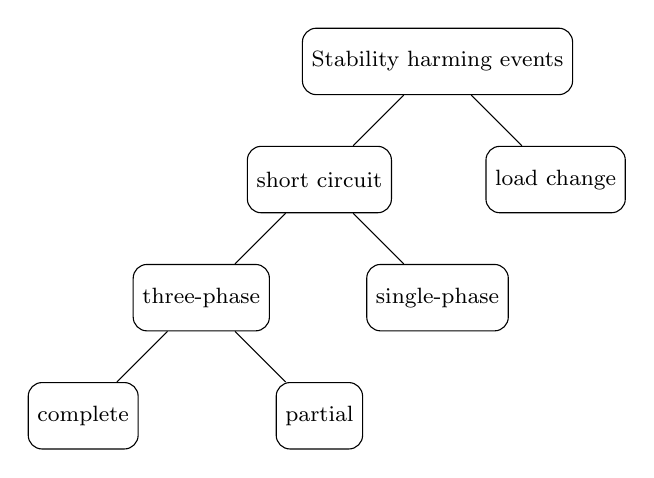
\begin{tikzpicture}[sibling distance=30mm, every node/.style={rectangle, draw, align = center, rounded corners=5pt, minimum height=24pt, font=\footnotesize}], %line width = 1, minimum width = 30mm, minimum height = 7mm,}]
                \node {Stability harming events}
                child {node {short circuit}
                        child {node {three-phase}
                                child {node {complete}}
                                child {node {partial}}}
                        child {node {single-phase}}}
                child {node {load change}};
        \end{tikzpicture}
        \caption{Overview of events harming the system stability of a power grid}
        \label{fig:stability-events}
\end{figure}

Events that can harm the system stability are sketched in \autoref{fig:stability-events}. This Student research paper~is interested in a three-phase short circuit, in the variants near a generator, far away of a generator and with a partial loss of a connecting overhead line.

%%%%%%%%%%%%%%%%%%%%%%%%%%%%%%%
\section{Numerical methods for TDSs and system modeling}
\commenting{
        \begin{itemize}
                \item \textbf{solving second order ODEs (explicit)}
                \item Differentiation explicit/impolicit, inertial value problems, boundary value problems, ...
        \end{itemize}
}

System dynamics is a method for describing, understand, and discuss complex problems in the context of system theory \textbf{[SOURCE]}. They often can be described through a set of coupled \acfp{ODE}, most resoluted in time dimension. \commenting{How to bridge towards different boundary types, explicit and implicit methods, ...; Different solving methods, ...} 

\acsp{ODE} can be solved through numerical integration with different methods. An easy and less complex method is Euler's method. It uses a linear extrapolation to calculate the functions value at the next timestep, so following the iterable function
\begin{align}
        f_\mathrm{t+1}=f_\mathrm{t}+\left(\frac{df}{dt}\right)_\mathrm{t} \cdot \Delta t \label{eq:euler},
\end{align}
with $t$ being the time and $f$ an on $t$ dependent function. Generally a system of second order \acsp{ODE} can be rewritten as two first order equations. This often simplifies the calculation or the use of numerical methods. The presented swing equation of a \acs{SG} in \autoref{eq:swing1} and \autoref{eq:swing2} has been split up by that principle.  

%%%%%%%%%%%%%%%%%%%%%%%%%%%%%%%
%%%%%%%%%%%%%%%%%%%%%%%%%%%%%%%
\chapter{Numerical modelling}
\label{chap:methods}

Following chapter will describe the implementation of Python Code for solving the derived \acs{ODE} system (see \autoref{sec:basics-sg}). For this the Python version 3.9 was used, in combination with the packages scipy, numpy, and matplotlib.\footnote{documentation and manual can be found on \href{https://scipy.org/}{\itshape https://scipy.org/} \autocite{virtanenSciPyFundamentalAlgorithms2020}, similiar for \href{https://matplotlib.org/}{\itshape matplotlib}, and \href{https://numpy.org/}{\itshape numpy} packages} The complete code is included in the \autoref{app:code}. % \mycomment[MK]{Write Chap Methods}

%%%%%%%%%%%%%%%%%%%%%%%%%%%%%%%
\section{Structure of the \acs{CCT} assessment}
\commenting{
        Program plan for determination / algorithm structure, containing:
        \begin{itemize}
                \item Pre questions:
                \begin{enumerate}
                        \item What do I want to know from the algorithm?
                        \item What do I want to see?
                \end{enumerate}
                \item Answers / Hints for the algorithm:
                \begin{enumerate}
                        \item What are needed inputs?
                        \item What are needed functions?
                        \item How do partial results interact with each other / puzzle together to the superior question?
                \end{enumerate}
        \end{itemize}
}

\begin{figure}[h]
        \centering
        \begin{tikzpicture}[node distance = 1.5cm, auto]
                % Place nodes
                \node [papStart] (Start1){Start};
                \node [papProcess, below of = Start1,label={[shift={(2.7,-0.6)}]\footnotesize\textit{label 1}}] (pro1){Prozess};
                \node [papProcess, below of = pro1,label={[shift={(3,-0.6)}]\footnotesize\textit{label 2}}](pro2){Prozess};
                \node [papDecision, below of = pro2, yshift= -9mm](dec1){Entscheidung};
                \node [papPredProc,  right of = dec1, xshift=25mm](predproc1){\nodepart{two}\shortstack{vordefinierter\\Prozess}};
                \node [papProcess, below of = predproc1,label={[shift={(2.3,-0.6)}]\footnotesize\textit{label 3}}](pro3){Prozess};
                \node [papEnd, below of = dec1, yshift= -20mm] (End) {Ende};
                
                % Place joins
                \coordinate [below of = dec1, yshift= -10mm] (join1);
                
                % Draw edges
                \path [papLine] (Start1) -- (pro1);
                \path [papLine] (pro1) -- (pro2);
                \path [papLine] (pro2) -- (dec1);
                \path [papLine] (dec1) -- node [right] {\papYes} (End);
                \path [papLine] (dec1) -- node [above] {\papNo} (predproc1);
                \path [papLine] (predproc1) -- (pro3);
                \path [papLine] (pro3) |- (join1);
        \end{tikzpicture}
        \caption{Program plan for determining the \acf{CCT}}
        \label{fig:program-plan}
\end{figure}

%%%%%%%%%%%%%%%%%%%%%%%%%%%%%%%
\section{Electrical simplifications and scenario setting}
\commenting{
        \begin{itemize}
                \item Simplification of all the components in SMIB network to a simple network
                \item Transforming into symmetrical components (for determination of shorts -> e.g. transformer)
        \end{itemize}
}

\subsection{Electric networks}

\subsection{Initial value calculation}
\commenting{
        \begin{itemize}
                \item Load flow analysis
                \item Calculation of $E_\mathrm{i}$, $I_\mathrm{i}$, $P_\mathrm{i}$, $\delta_\mathrm{i}$, ..., as well for IBB
        \end{itemize}
}

%%%%%%%%%%%%%%%%%%%%%%%%%%%%%%%
\section{Implementation of the time domain solution}
\label{sec:tds}

\commenting{
        \begin{itemize}
                \item Different levels of TDS; With/without solving of algebraic equations at each timestep; With/without calculation of turbine momentum at each timestep (dependent on omega)
                \item Utilization as a function: calculation with clearing and without clearing: for determination of CCT needed
        \end{itemize}
}

%%%%%%%%%%%%%%%%%%%%%%%%%%%%%%%
\section{Implementation of the equal area criterion}

\commenting{
        \begin{itemize}
                \item Iterative process needed? Due to omega and delta dependencies of $P_e$ and $P_m$
                \item Different methods of CCT calculation: P-$\delta$-curve; P-t-curves
        \end{itemize}
}

\section{Implementation of helping functions}


%%%%%%%%%%%%%%%%%%%%%%%%%%%%%%%
%%%%%%%%%%%%%%%%%%%%%%%%%%%%%%%
\chapter{Results}
\label{chap:results}

% \mycomment[MK]{Write Chap Results}

%%%%%%%%%%%%%%%%%%%%%%%%%%%%%%%
\section{Analytical results}

%%%%%%%%%%%%%%%%%%%%%%%%%%%%%%%
\section{Numerical results}

%%%%%%%%%%%%%%%%%%%%%%%%%%%%%%%
\section{Discussion}
\label{sec:discussion}

% \mycomment[MK]{Write Sec Discussion}